\section{Design And Implementation}
\label{sec:design}

\subsection{Overview}
\label{subsec:overview}
This idea was tested using a synthetic benchmark application written by the authors.  The benchmark consists of two executables: the main application which uses MPI and simulates the I/O patterns of a typical HPC application and a daemon process that is started on each compute node.  The daemon has two tasks: manage the GPU memory and copy data from GPU memory out to a file.  Note that the daemon does \emph{not} copy the data into the GPU memory; that is handled by the individual ranks of the main application.   There needs to be exactly one daemon process on each compute node regardless of how many MPI ranks are running on each node.  \footnote{Due to the limitations of aprun, starting this daemon is somewhat involved.  See section \ref{subsec:cray-specific}.}

With the daemon process running on each node, the application begins its main execution.  In this case, since it's just a synthetic 
I/O benchmark, it performs no actual computation; it simply writes a specified amount of data and then sleeps for a specified amount of time.  For these tests, the sleep time was deliberately calculated to allow enough time for the data in GPU memory to drain.
\subsection{Communication Between the Application and Daemon}
\label{subsec:comm}

Communication between the main application and the daemon happens over two different channels.  Short messages for coordination between the application and the daemon are handled using the Common Communication Interface (CCI).\cite{atchley11:cci}  Bulk data is copied to and from GPU memory using \texttt{cudaMemcpy()}.

\begin{figure*}[hp]
\centerline{
  \subfloat[Application sends write request message to daemon]{
    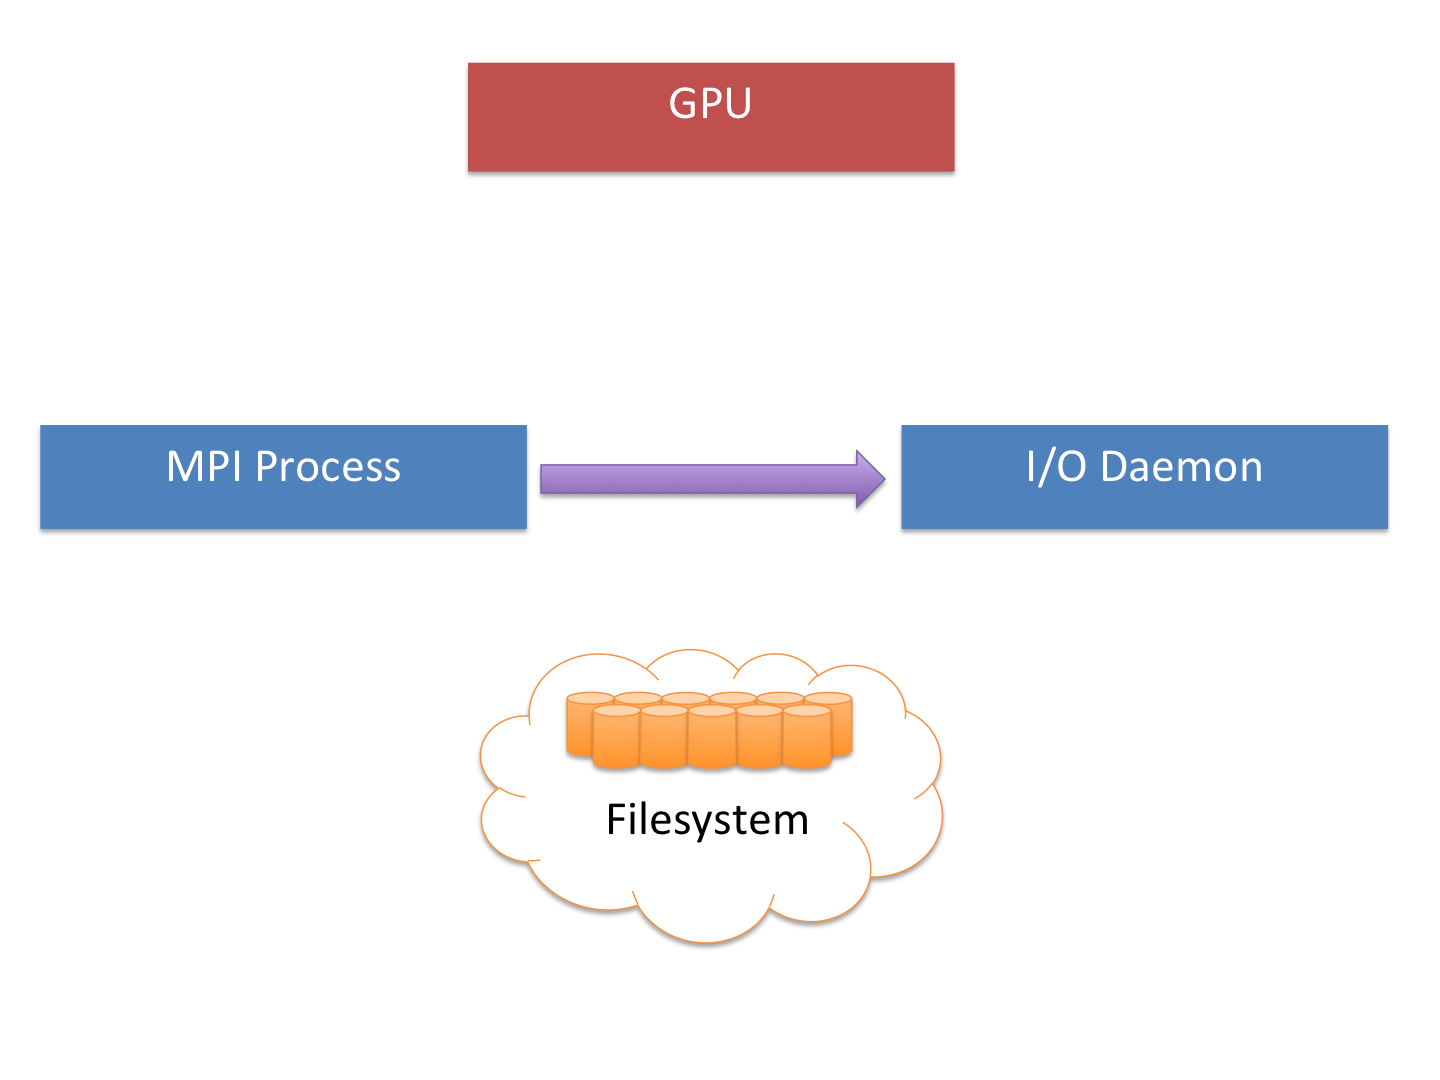
\includegraphics[width=2.5in]{figures/Data_Movement/Slide09}%
    \label{fig:comm_a}}
  \hfil
  \subfloat[Daemon allocates GPU memory and converts pointer into IPC handle]{
    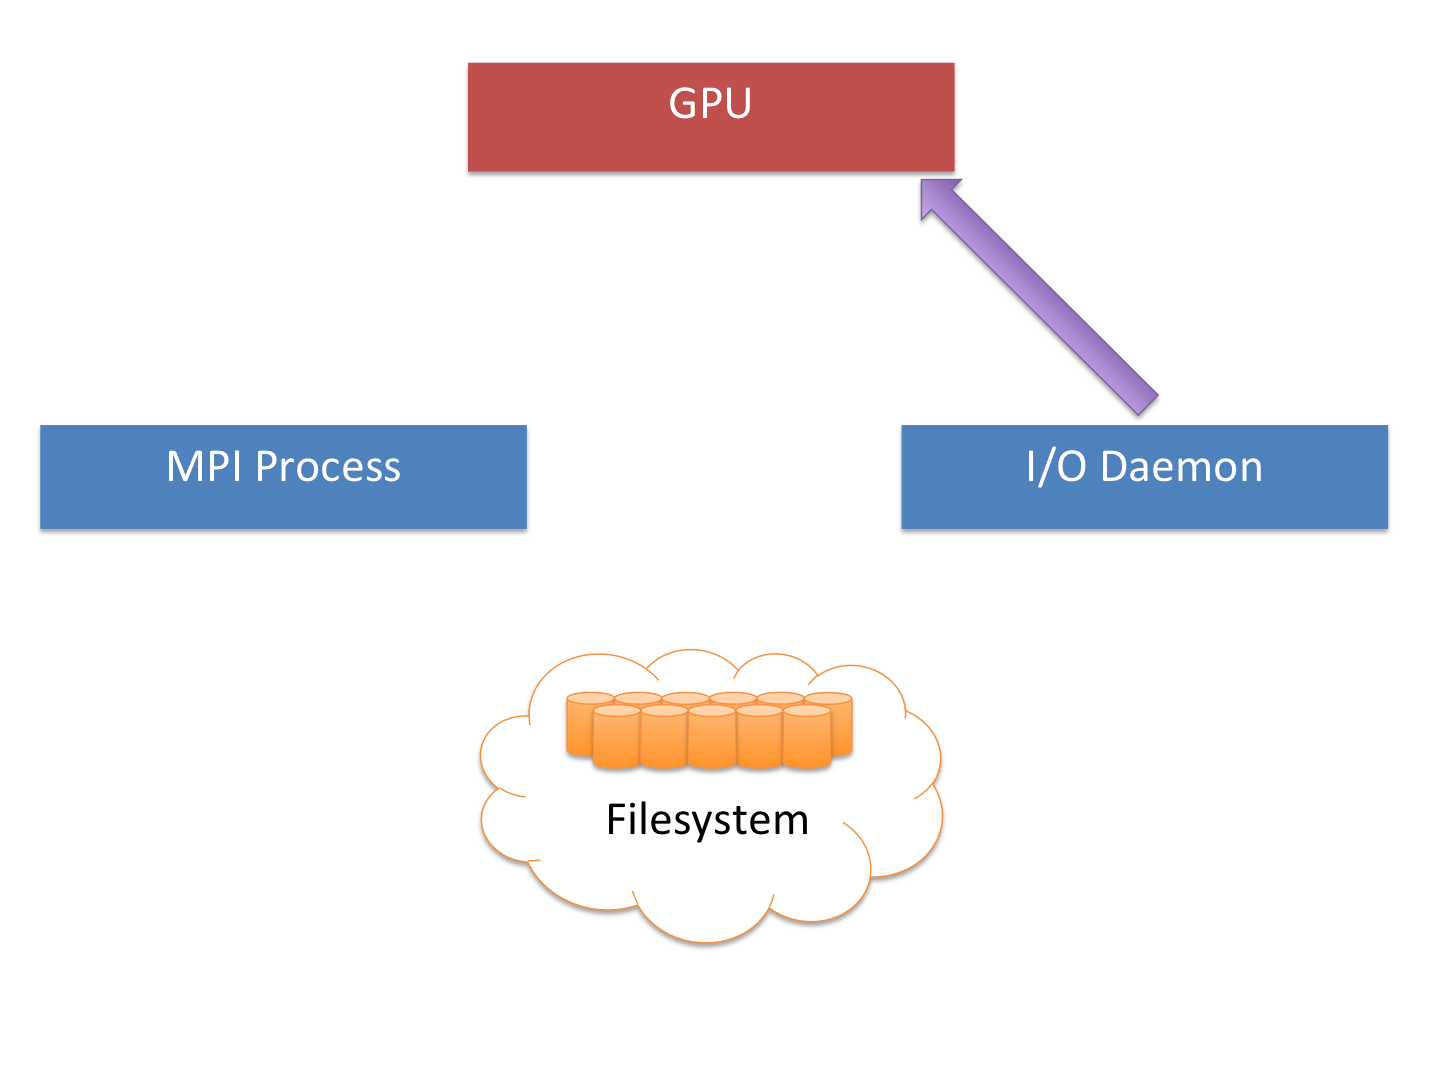
\includegraphics[width=2.5in]{figures/Data_Movement/Slide10}%
    \label{fig:comm_b}}}
\centerline{
  \subfloat[Daemon sends reply message with IPC handle]{
    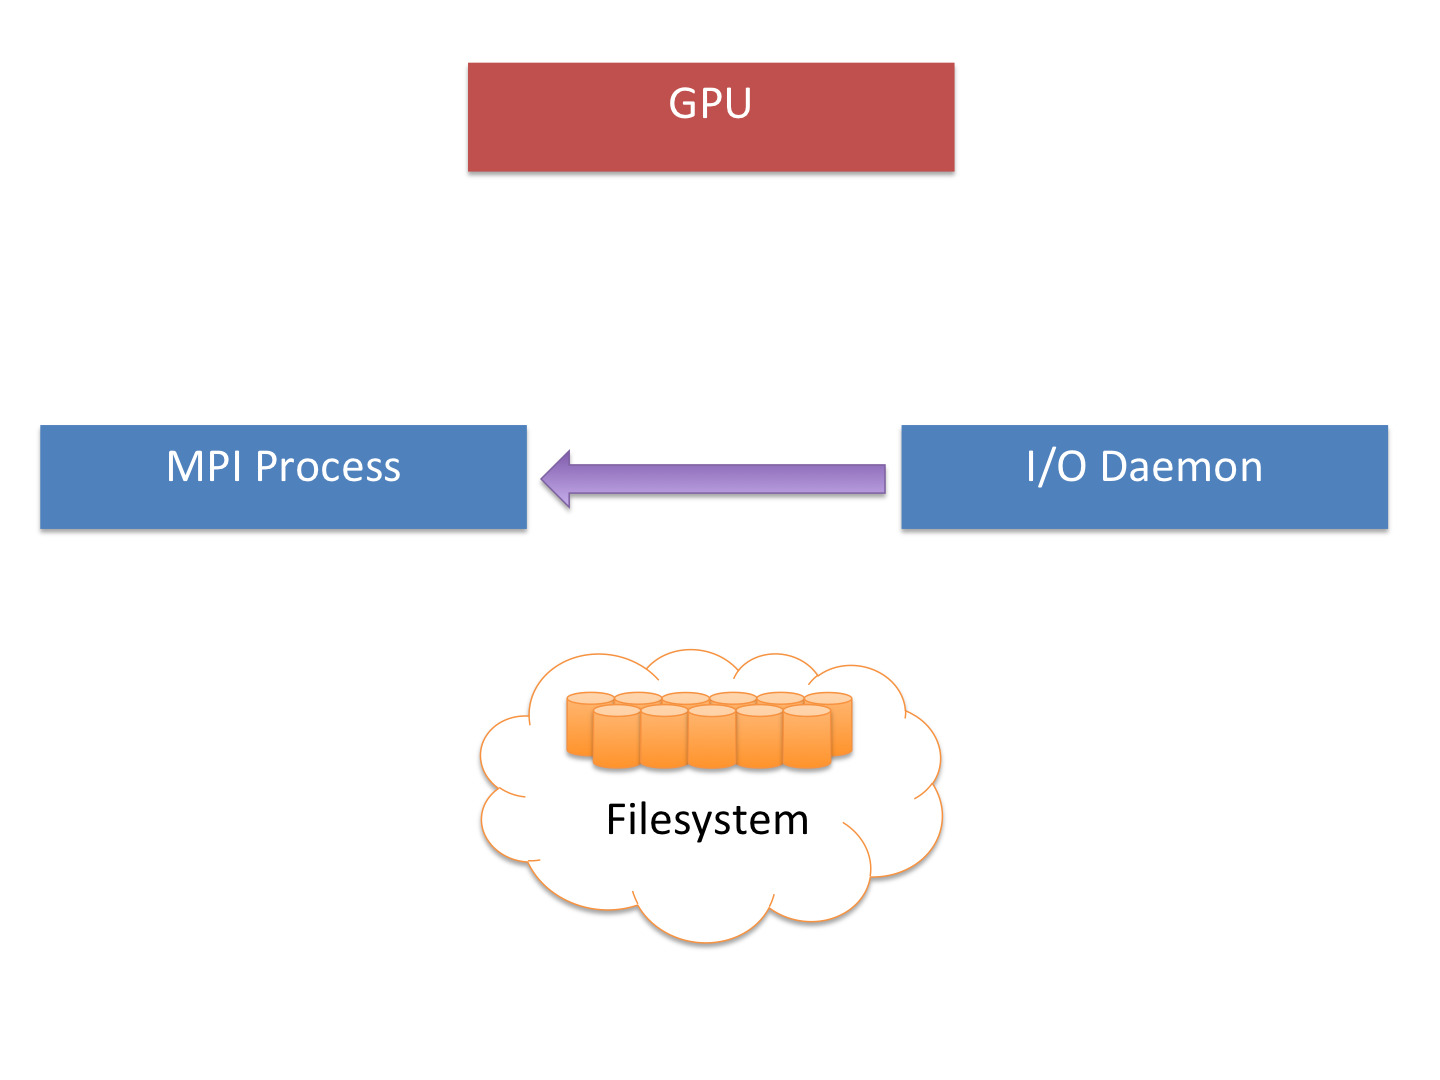
\includegraphics[width=2.5in]{figures/Data_Movement/Slide11}%
    \label{fig:comm_c}}
  \hfil
  \subfloat[Application writes data to GPU memory]{
    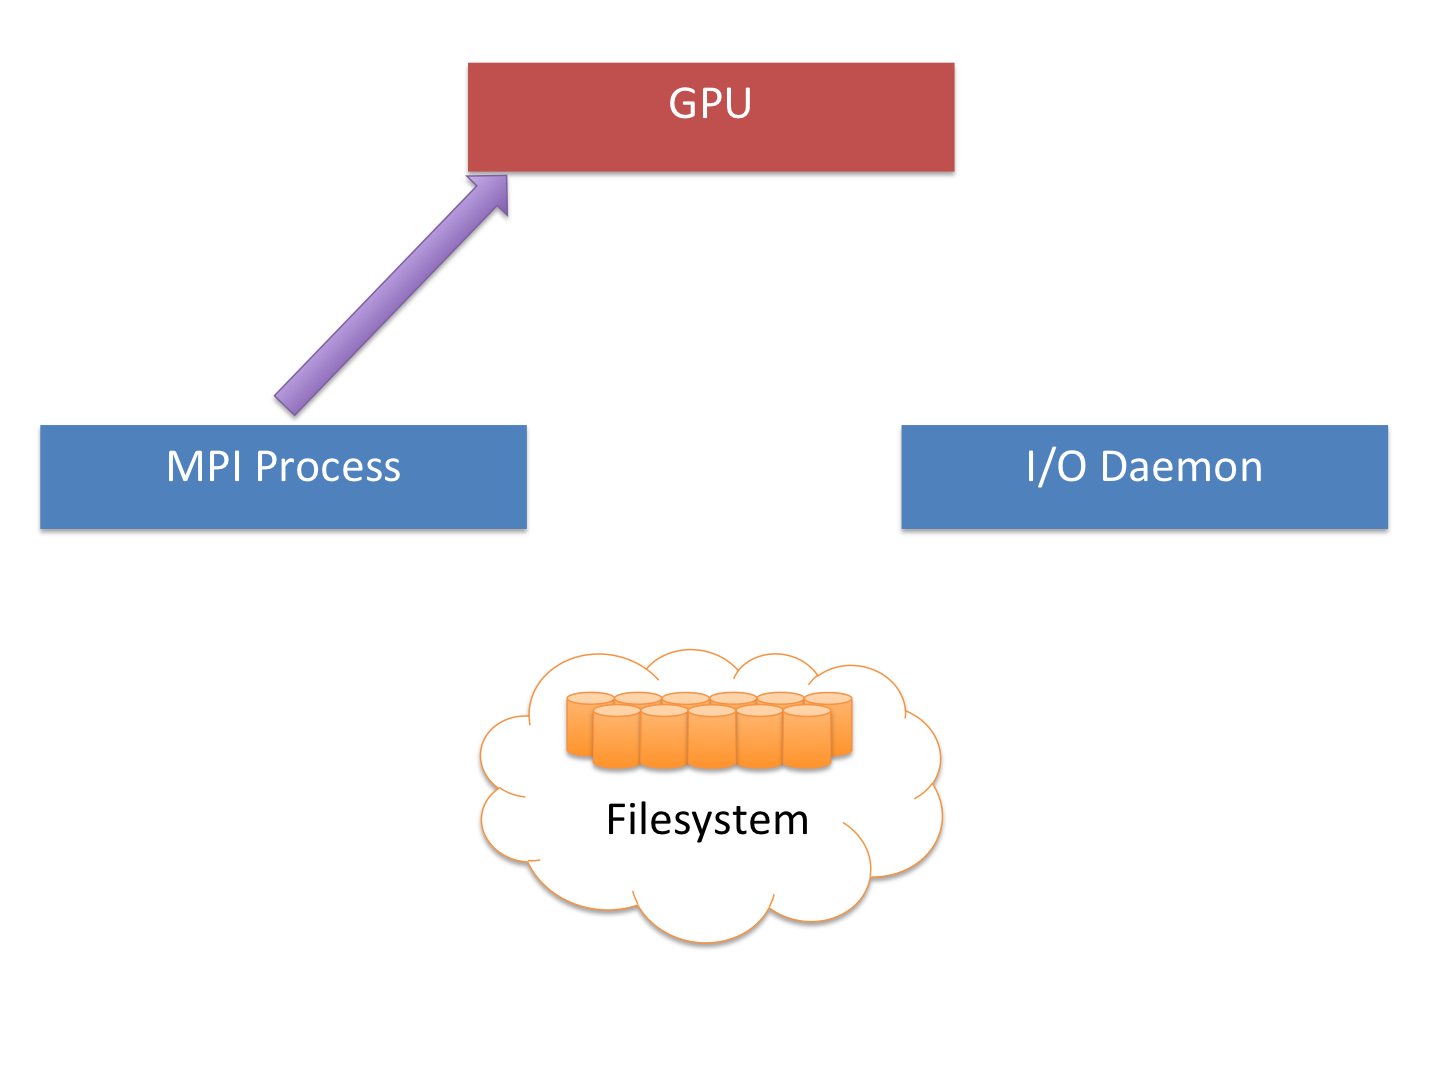
\includegraphics[width=2.5in]{figures/Data_Movement/Slide12}%
    \label{fig:comm_d}}}    
\centerline{
  \subfloat[Application sends write complete message to daemon]{
    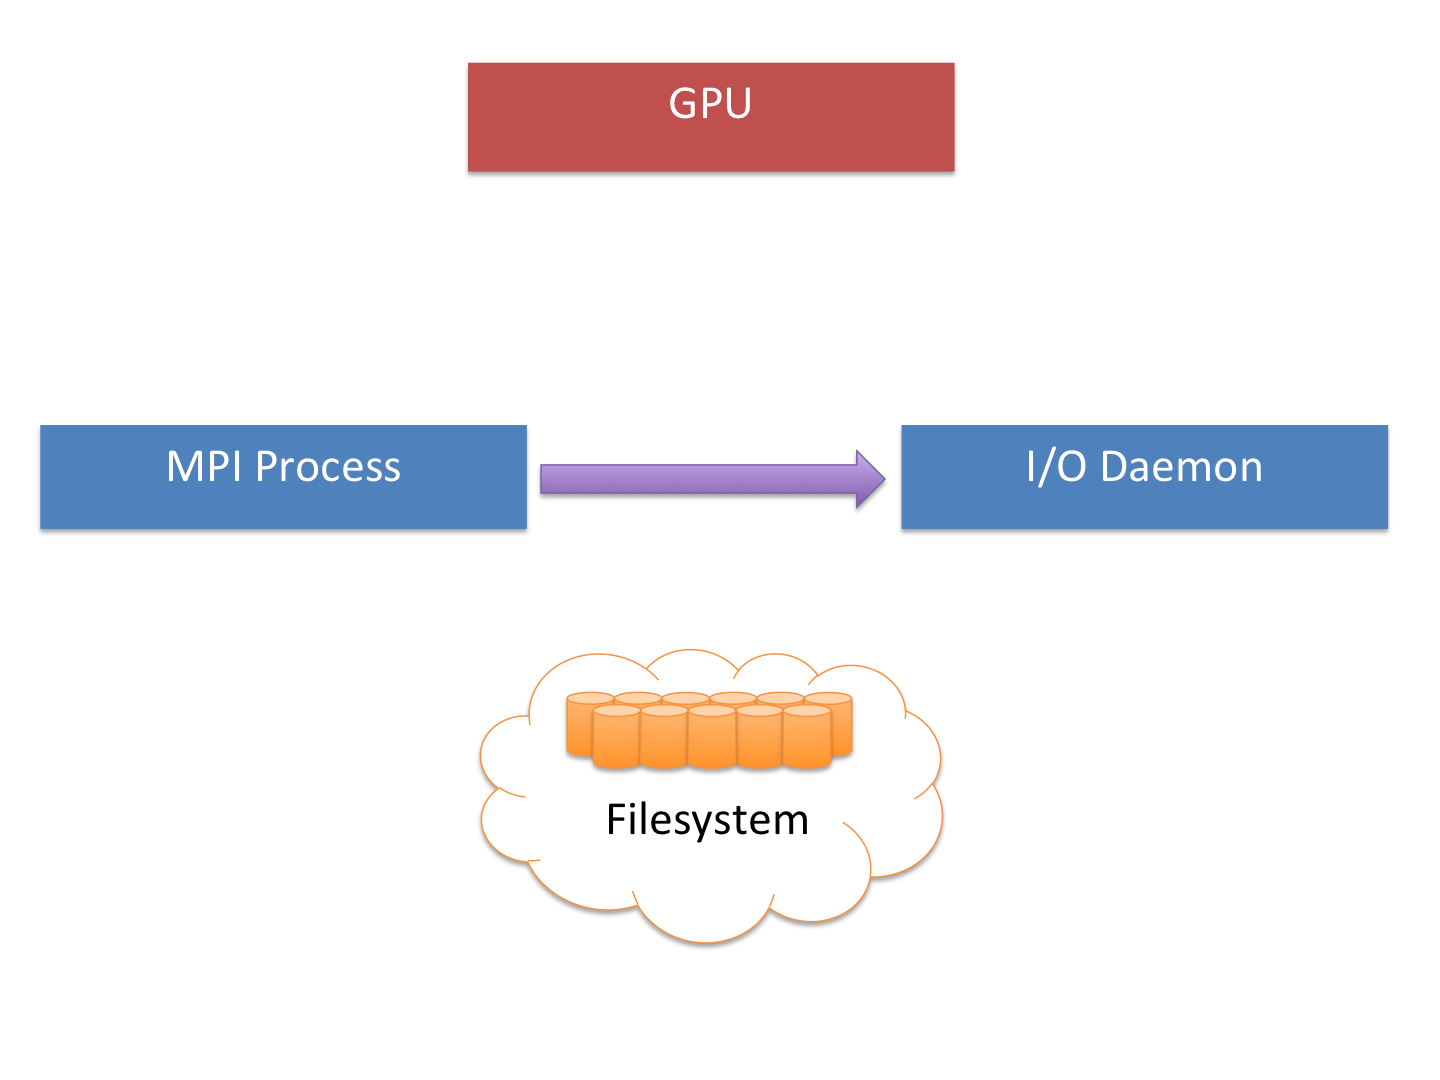
\includegraphics[width=2.5in]{figures/Data_Movement/Slide13}%
    \label{fig:comm_e}}
  \hfil
  \subfloat[Daemon copies data from GPU memory to system memory]{
    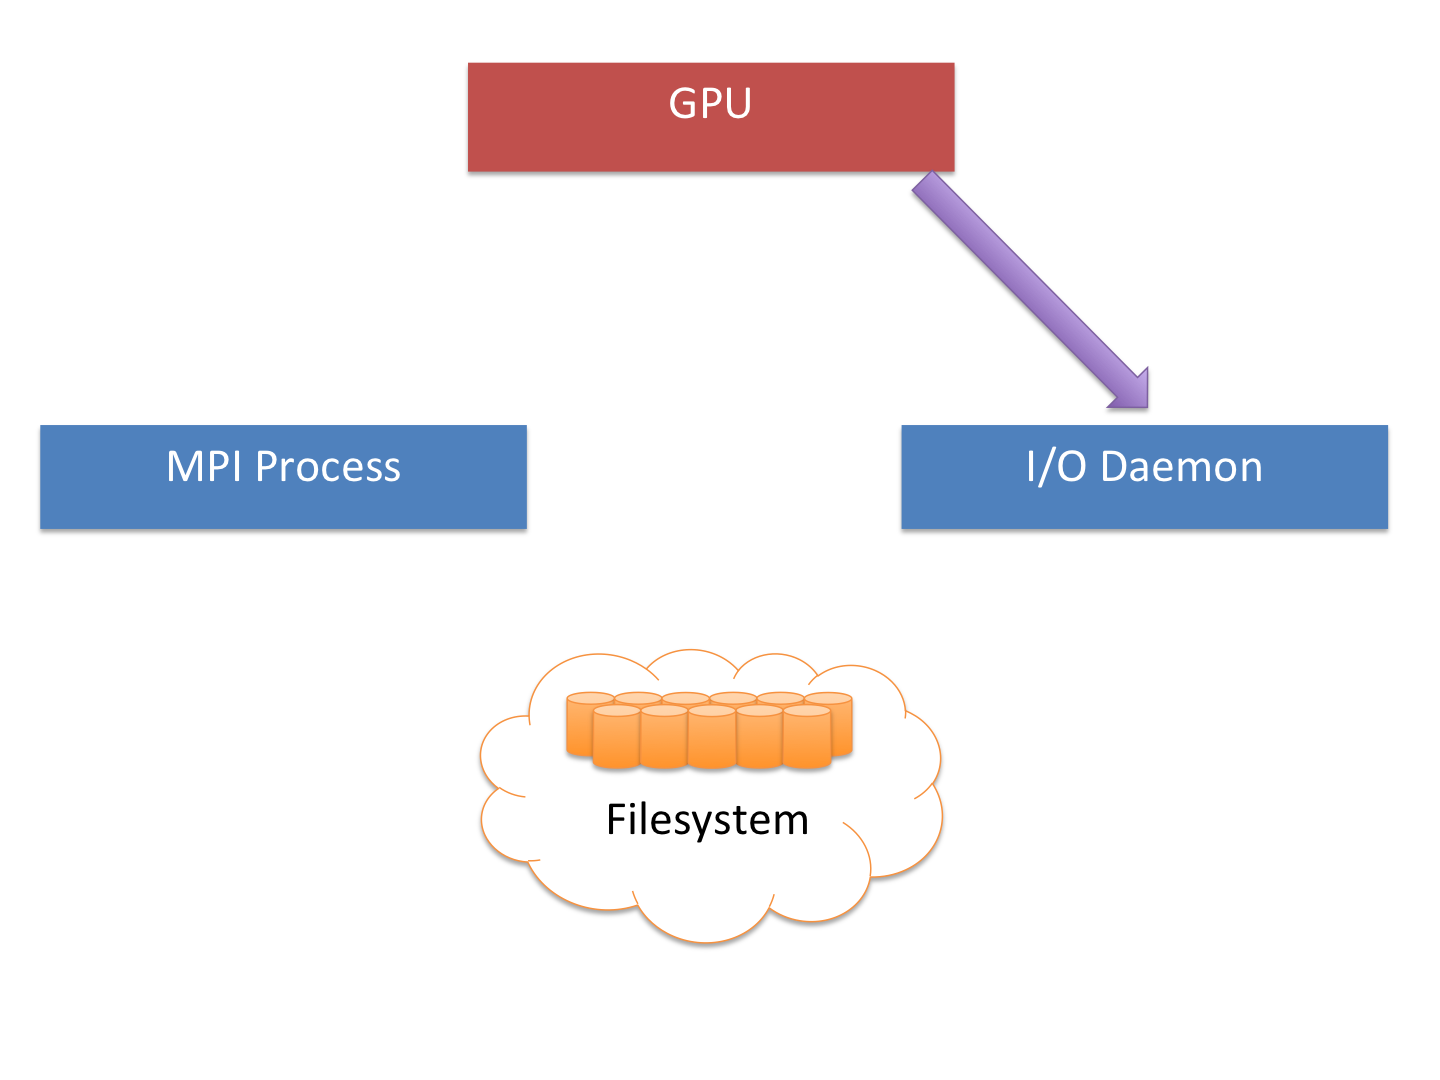
\includegraphics[width=2.5in]{figures/Data_Movement/Slide14}%
    \label{fig:comm_f}}} 
\centerline{
  \subfloat[Daemon writes data to filesystem]{
    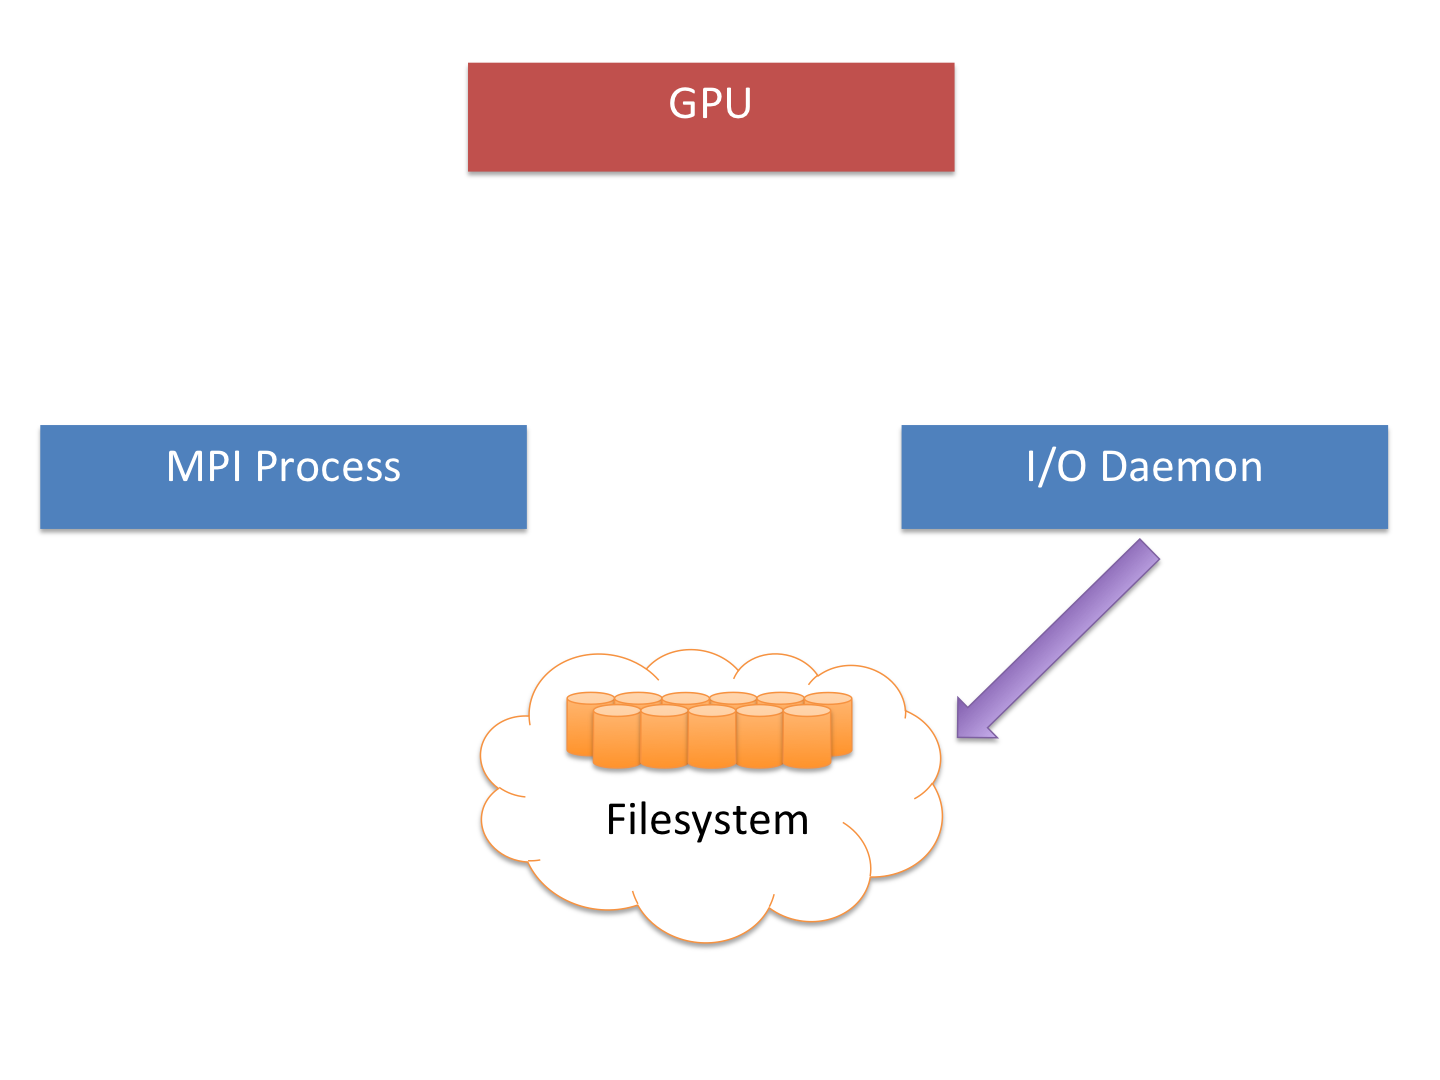
\includegraphics[width=2.5in]{figures/Data_Movement/Slide15}%
    \label{fig:comm_g}}} 
\caption{Communications steps}
\label{fig:communications}
\end{figure*}


Writing data from the application is a seven step process.

When it's time to write, the application sends a short message to the daemon using CCI.  This message is a request to write data, and contains the amount of data and the starting offset into the output file.\footnote{For this benchmark, the daemon names output files based on the MPI rank of the requestor.  For production code, something more flexible will obviously be needed.}(Figure \ref{fig:comm_a})

When the daemon receives this message, it will attempt to allocate memory on the GPU.  Assuming the allocation succeeds, the daemon will use \texttt{cudaIpcGetMemhandle()} to create a memory handle for the allocation. (Figure \ref{fig:comm_b})

The daemon will then reply to the application with the size of memory that was actually allocated and the memory handle that the application can use to access the GPU memory.  Note that the size value may be less than what the application asked for. (Figure \ref{fig:comm_c})

Upon receiving the reply, the application opens the memory handle and converts it back to a standard pointer.  The application then uses \texttt{cudaMemcpy()} to copy the specified amount of data up to the GPU memory. (Figure \ref{fig:comm_d}) 

When the copy has completed, the application closes the memory handle and sends a message back to the daemon saying that this particular write has completed.  (Figure \ref{fig:comm_e})  If the application has more data to write, it can repeat the previous steps, or else it can continue with its calculations.

Note that at this point the data has not made it out to the filesystem yet; it's just sitting in GPU memory.  

The daemon maintains a pair of lists.  One list is the blocks of GPU memory that have been assigned to the ranks of the main application, and which the ranks are presumably copying data into.  The second list is for all the blocks of memory for which the `write complete' message (step e) has been received.  When the daemon thread that handles CCI messages receives a `write done' message for a block, it moves that block from the first list to the second list.  It then notifies the background write thread(s) that the block is now ready to be written to the filesystem.

The daemon maintains one or more background threads that are responsible for copying data out of GPU memory into normal system memory and then writing that data to the filesystem.  These threads allow the writes to the filesystem to happen asynchronously while the main thread handles all the CCI messages.  Since it's impossible to write directly from GPU memory to the filesystem, each thread will copy a block of data from GPU memory into a buffer in main memory.  (Figure \ref{fig:comm_f})  It will then write the data to the output file at the location specified in the original request message.  (Figure \ref{fig:comm_g})  Once data has been written to the filesystem, the write thread free's the GPU memory so that it can be used in another request.

\begin{figure}
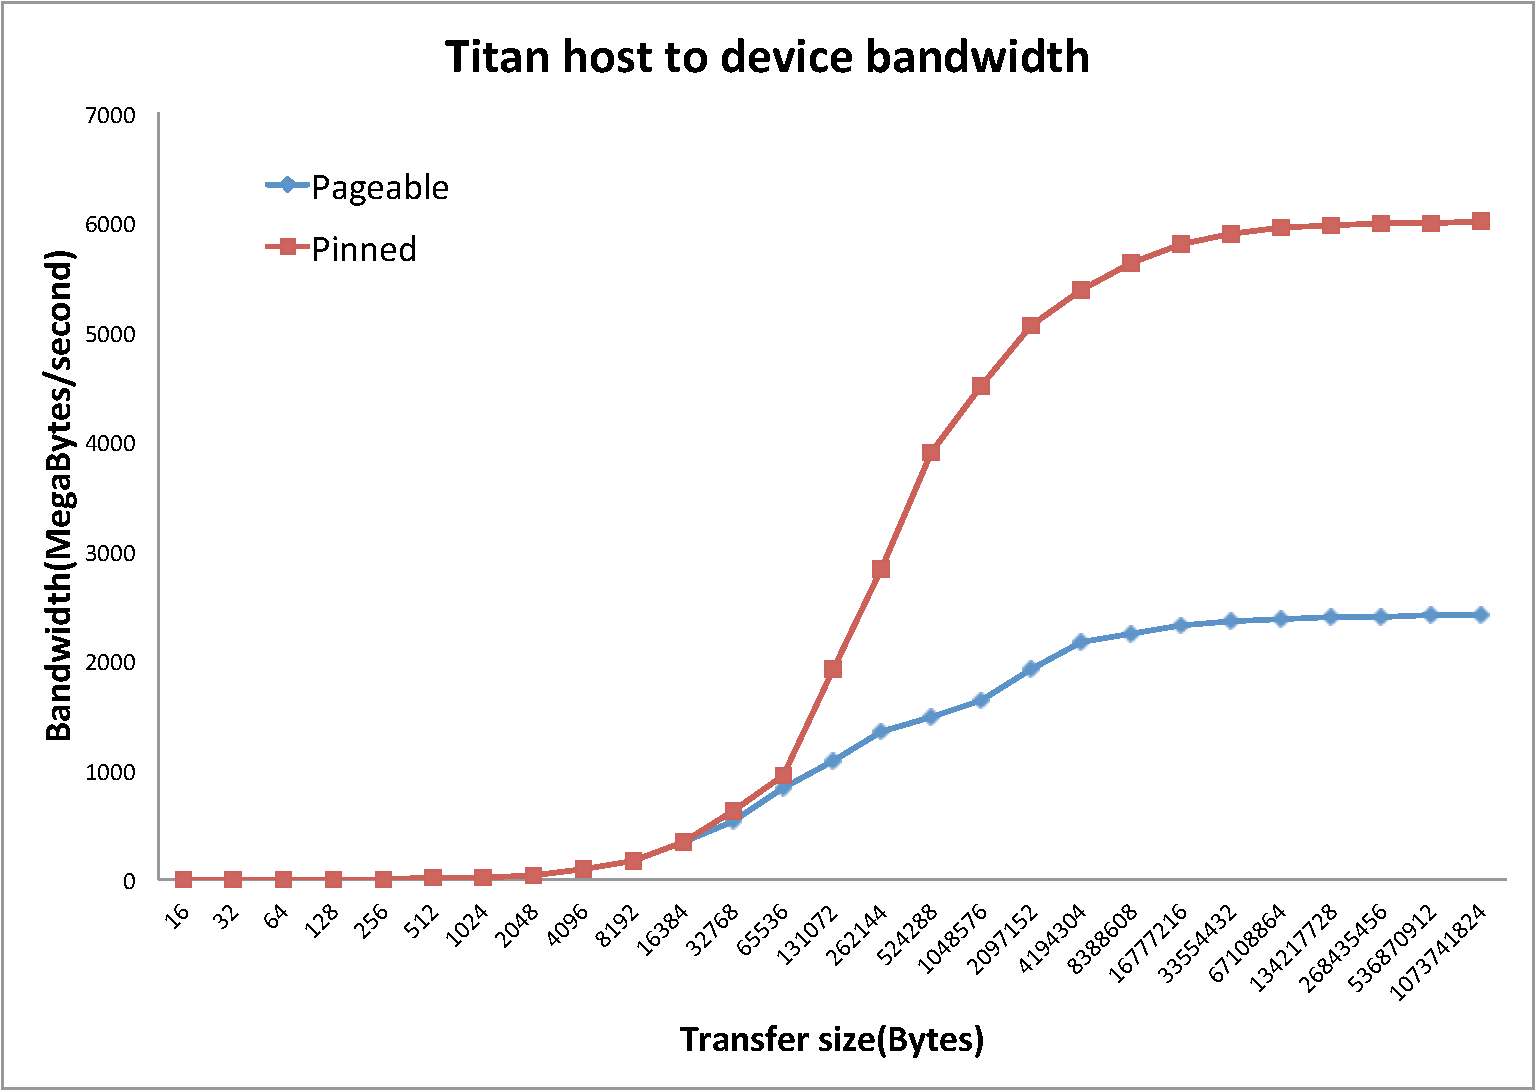
\includegraphics[width=\linewidth]{figures/Host2Device_BW.pdf}
\caption{Bandwidth between system memory and GPU memory as a function of write size\cite{ac_guide}} 
\label{fig:transfer_bw}
\end{figure}

Note that each write thread in the daemon has its own buffer in system memory.  Each of these buffers is deliberately kept fairly small - 16MB - in order to conserve resources.  Testing done on Titan shows that 16MB block sizes are large enough for \texttt{cudaMemcpy()} to give good performance.\cite{ac_guide}  Larger buffers would simply use up memory without improving performance noticeably. See Figure \ref{fig:transfer_bw}.

Also note that the daemon limits the amount of memory allocated to any single request to 16MB.  This was done to provide some limited load-balancing.  If an application wants to write 512MB, it will therefore have to make 32 separate requests.  If other ranks on the node are trying to write at the same time, their requests will all be interleaved and hopefully no rank will be starved out.


\subsection{Cray-Specific Details}
\label{subsec:cray-specific}

There are a few peculiarities of the Cray environment that need to be taken in to account in order for this software to work properly.  The first peculiarity has to do with limiting access to the GPU and associated hardware.  The CUDA runtime can be configured to limit access to the GPU to a single thread, to multiple threads from a single process or to multiple threads from multiple processes.  On Titan, if no special options are given to qsub, the CUDA runtime will be configured for a single thread.  Since software described in this paper requires access to the GPU from multiple processes, users must switch to the appropriate compute mode.  This is done by passing the flag "-l feature=gpudefault" to qsub.\footnote{It may seem strange to have to explicitly switch to a mode called 'gpudefault'.  The naming scheme comes from the CUDA documentation.  On a standard CUDA install, the GPU would in fact default to allowing access from multiple processes.  Titan is configured differently, however.  Thus the need to explicitly tell qsub to switch the GPU's to the `default' mode.}

The second peculiarity has to do with actually starting the daemon process.  Normally, executables are started on the compute nodes by aprun.  However, aprun is designed to start a single executable, not to start two different executables.  Even in MPMD mode, it won't start two different executables on the same node.  The solution is to have one rank on each node call \texttt{fork()} and then \texttt{execve()}.  Since MPI purposely hides the compute topology from the application, deciding exactly which ranks call fork() takes a little more work.  Specifically, all ranks will attempt to open a file using the \texttt{O\_CREAT} and 
\texttt{O\_EXCL} flags.  The name of the file is taken from the compute node's host name.  This combination of flags and filename ensures that exactly one rank on each node successfully opens the file.  The ranks that succeed will then start the daemon processes.

%
% Everything below is commented out.  It's text I've toyed with using, but decided not to for whatever reason
%
\begin{comment}


It's debatable whether this sort of load balancing is necessary or even desirable.  Indeed, preliminary testing seemed to indicate that it might be faster to let the daemon allocate  as much GPU memory as the client requested (assuming there was enough free).  However, that same testing showed that one of the CUDA functions - \texttt{cudaIpcOpenMemHandle()} - became unreliable once GPU memory allocations exceeded 512MB.  Until the nature of that problem could be determined, it was decided to limit allocations to 16MB.



CUDA has several functions for facilitating interprocess communications.  Among other things, one can convert a device pointer to a process-independant memory handle.  Another process can take that memory handle and convert it back to a device pointer.


\end{comment}

